% \documentclass[a4paper]{article}
% \usepackage[ngerman]{babel}
% \usepackage[utf8]{inputenc}
% \usepackage[top=2.5cm,bottom=1.75cm,right=2cm,left=2.3cm]{geometry}
% \usepackage{wrapfig}
% \usepackage{floatflt}
% \usepackage{graphicx}
% \usepackage[colorlinks=true,linkcolor=black,bookmarksnumbered=true,breaklinks=true,pdfstartview=FitH]{hyperref}
% 
% \title{\textbf{Praktikum 9} \\ ~ \\Ultraschall I}
% 
% \author{Michael Kopp}
% 
% \date{18. Oktober 2007}
% 
% %2007-11-04 12:25
% 
% 
% \begin{document}
% 
% 
% \maketitle


\section{Beugung am Doppelspalt}


\subsection{Versuch}

\begin{figure}
	\centering
   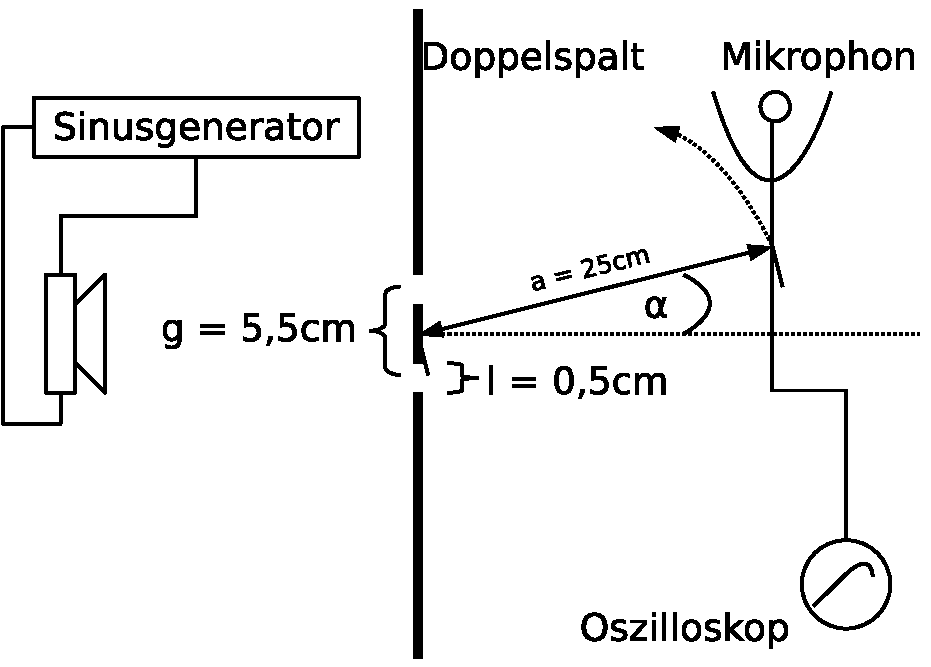
\includegraphics[width=0.8\textwidth]{praktika/mat_praktika/doppelspalt}
   \caption{Aufbau des Doppelspaltversuchs}
\end{figure}



Vor einen Doppelspalt aus Plastik wird eine Ultraschallsender in ca. \(20cm\) Abstand zwischen den beiden Spalten positioniert. Dies dient dazu, dass die Schallwellen, die auf die Spalte treffen eine feste Phasenbeziehung haben - steht der Sender genau zwischen den beiden Spalten (das wäre der Idealzustand), haben die Schallwellen, die von den Spalten ausgehen die Phasendifferenz \(\Delta \varphi = 0\).

Hinter dem Doppelspalt wird nun ein Mikrophon im Abstand von \(a = 25cm\)\footnote{Gemessen zum Mittelpunkt zwischen den beiden Spalten} halbkreisförmig bewegt\footnote{Dabei muss man sehr vorsichtig vorgehen, weil schon die Bewegung des Mikrophons zu Einer veränderten Anzeige führt; präzise Messungen können so nur bei \emph{ruhendem} Mikrophon vorgenommen werden.}. Über ein Oszilloskop wird überwacht, was das Mikrophon empfängt. Erkennt man auf dem Oszilloskop ein Minimum der vom Mikrophon registrierten Schallwellen\footnote{Eigentlich Minimum an registriertem \emph{Druck}; schließlich ist das Mikrophon druckempfindlich.}, so misst man den Winkel \(\alpha\) den der Lautsprecher zu einer gedachten Geraden senkrecht zum Doppelspalt durch den Mittelpunkt der Doppelspalte einschließt.

Dann gilt es, die Eigenfrequenz des Mikrophons zu ermitteln; offensichtlich nimmt es Frequenzen innerhalb eines kleinen Bereiches wesentlich besser war. Dazu wird das Mikrophon direkt vor den Lautsprecher gestellt und am Frequenzgenerator wird so lange de Frequenz verstellt, bis das Oszilloskop einen maximalen Ausschlag anzeigt. Bei uns ergab sich das für eine am Oszilloskop ablesbare Periodendauer von \(T = 24\mu s\); also bei einer Frequenz von \(f = \frac{1}{T} = 41 \frac{2}{3} kHz\). Über den Zusammenhang
\begin{equation}
   c = \frac{\lambda}{T} = \lambda \cdot f
   \label{eq_c=lf_p}
\end{equation}
ergab sich da \(c = 340 \frac{m}{s}\) eine Wellenlänge von \(\lambda \approx 8,16mm\).






\subsection{Beobachtungen}


``Lokale'' Maxima, bei denen der Ausschlag kleiner ist als in ihrer Umgebung, finden sich für folgende Winkel: 
\[ \alpha = \left \{   0^o; 11^o; 20^o; 27^o; 40^o; 50^o; 61^o  \right \} \]
Je größer der Winkel \(\alpha\) dabei ist, desto weniger Eindeutig ist das Maximum - also umso kleiner sind die im Oszilloskop beobachteten Wellenhöhen\footnote{Wellen, die man im Oszilloskop sieht}.


\subsection{Auswertung}


Maxima ergeben sich überall dort, wo der Gangunterschied der beiden von den Doppelspalten weglaufenden Wellen 
\begin{equation}
	\delta = k \cdot \lambda ~~ k = (0; 1; 2; ...)   
	\label{eq_gangunterschied}
\end{equation}
beträgt; an dieser Stelle haben die beiden Wellen, die von den Spalten ausgehen und sich zur gemessenen Welle addieren den Phasenunterschied \(\Delta \varphi = 0\); es gilt nämlich
\begin{equation} 
   \frac{\Delta \varphi}{2 \cdot \pi} = \frac{\delta}{\lambda}
   \label{eq_zshg_gangunterschied-phasendiffernz}
\end{equation} 
Im Zeigermodell addieren sich somit zwei parallele Zeiger zu einem resultierenden, der somit logischerweise die maximale durch Addition erreichbare Länge hat.


In unserem Versuch gilt der Zusammenhang \(a \gg g\) näherungsweise. Somit haben die im Mikrophon eintreffenden Schallwellen einen nahezu parallelen Weg zurückgelegt und somit kann man näherungsweise sagen, dass gilt:
\begin{equation}
   \delta = g \cdot sin( \alpha )
   \label{eq_fraunhofer_gangunterschied}
\end{equation}
Da sich die Gangunterschiede, bei denen sich Maxima ergeben nach Formel \ref{eq_gangunterschied} berechnen lassen, kann man Formel \ref{eq_fraunhofer_gangunterschied} und Formel \ref{eq_gangunterschied} kombinieren und es ergibt sich die sog. \textsc{Fraunhofer} Näherung (siehe Kap. \ref{fraunhofer_naehrung} auf S. \pageref{fraunhofer_naehrung}):
\begin{equation}
   g \cdot sin( \alpha ) = k \cdot \lambda \Rightarrow asin\left ( \frac{k \cdot \lambda}{g}\right )   ~~ k = (0; 1; 2; ...)   
\end{equation}
Danach ergeben sich für Maxima \(k\). Ordnung die Winkel in Tabelle \ref{tab_alpha_k} auf S. \pageref{tab_alpha_k}

\begin{table}
\centering
\begin{tabular}{l|l|l|l}
\(k\) &~~~ \(\alpha_k errechnet\) [\(^o\)] &~~~ \(\alpha_k gemessen\) [\(^o\)] &~~~ \(prozentuale Abweichung\) \\
\hline
0	&~~~	0	&~~~	0	&~~~	0\\
1	&~~~	8,53	&~~~	11	&~~~	-28,92\\
2	&~~~	17,26	&~~~	20	&~~~	-15,87\\
3	&~~~	26,43	&~~~	27	&~~~	-2,16\\
4	&~~~	36,4	&~~~	40	&~~~	-9,88\\
5	&~~~	47,89	&~~~	50	&~~~	-4,41\\
6	&~~~	62,9	&~~~	61	&~~~	3,01\\
\end{tabular}
\caption{Vergleich gemessener und errechneter Werte für \(\alpha\)}
\label{tab_alpha_k}
\end{table}



Für die von uns gemessenen Winkel ergeben sich so bei den einzelnen Maxima die Wellenlängen in Tabelle \ref{tab_lambda_k} auf S. \pageref{tab_lambda_k}

\begin{table}
\centering
\begin{tabular}{l|l|l|l}
\(k\)	&~~~	\(\alpha_k gemessen\) [\(^o\)]	&~~~	\(\lambda_k errechnet\) [mm]	&~~~	\(Prozentuale Abweichung\)\\
\hline
1	&~~~	11	&~~~	10,49	&~~~	-28,61\\
2	&~~~	20	&~~~	9,41	&~~~	-15,26\\
3	&~~~	27	&~~~	8,32	&~~~	-2\\
4	&~~~	40	&~~~	8,84	&~~~	-8,31\\
5	&~~~	50	&~~~	8,43	&~~~	-3,27\\
6	&~~~	61	&~~~	8,02	&~~~	1,75\\
\end{tabular}
\caption{Vergleich gemessener und errechneter Werte für \(\lambda\)}
\label{tab_lambda_k}
\end{table}


Es ergeben sich also besonders für große Winkel eine große Übereinstimmung der gemessenen und errechneten Werte.


\subsection{Mögliche Erklärungen für die Abweichungen}
\label{kap_abw01}


 Möglichkeiten für die Abweichungen können sein:
\begin{description}
   \item[Winkel] Die Winkel mussten mit einem Geodreieck abgemessen werden und es war leider zu kurz, um die Punkte, zwischen denen gemessen werden musste zu erreichen. Es musste also mehr oder weniger geschätzt werden.
   
   \item[Bestimmung der Punkte] Es war nicht ganz klar, zwischen welchen Punkten der Winkel überhaupt zu messen war; schließlich hätte man den soliden Fuß des Mikrophons unsichtbar und durchlässig machen müssen, um ihn zu erreichen...
   
   \item[Bestimmung eines Maximums] Bei der Entscheidung, ob es sich an entsprechender Stelle um ein Maximum handelte oder nicht hatte man bei der Untersuchung viel eignende Ermessensspielraum, ob es sich an besagter Stelle sicher um ein Maximum handelte oder nicht.
   
   \item[Wellenlänge] Die Wellenlänge haben wir errechnet in dem wir die Periodendauer vom Oszilloskop abgelesen haben - hier sind falsche Ablesungen möglich - außerden haben wir die ``standardisierte'' Schallgeschwindigkeit \(c = 340\frac{m}{s} \) verwendet, die aber bei uns sicher nicht galt (schließlich ist sie temperaturabhängig).
   
   \item[Fraunhofer Näherung] Die \textsc{Fraunhofer}-Näherung gilt eigentlich nur für sehr große Abstände von Mikrophon und Doppelspalt; möglicherweise war der unsrige zu klein...
\end{description}



		\subsection{\textsc{Fraunhofer}-Näherung} 
		\label{fraunhofer_naehrung}
Gilt bei der Beugung am Doppelspalt
\begin{equation}
a \gg g\\
 	\label{eq_aggg_p}
 \end{equation}
 \begin{equation}
a \gg d_k
 	\label{eq_aggdk_p}
\end{equation}
so kann man sich einigen Rechenaufwand sparen. Durch Formel \ref{eq_aggg_p} ist nämlich der Winkel \(\alpha_k\) nicht nur unter der Linie vom Punkt zwischen den Spalten zum Punkt auf den Leuchtschirm und der Horizontalen zu finden sondern auch näherungsweise zwischen den beiden Lichtstrahlen und einer gedachten Waagerechten. Außerdem sind die beiden Lichtstrahlen dadurch praktisch parallel und (nur) deswegen kann man den Winkel \(\alpha_k\) direkt an den Spalten wiederfinden (S. Skizze in Abbildung \ref{img_beugungamdoppelspalt_p} auf Seite \pageref{img_beugungamdoppelspalt_p}). Dadurch ergibt sich ein ähnliches Dreieck\footnote{Der Winkel \(\alpha_k\) und ein rechter Winkel findet sich sowohl in den kleinen Dreieck am Doppelspalt (in der Skizze teilweise. fein gestrichelt und fett) als auch in dem Dreieck, mit dem \(\alpha_k\) bestimmt wird (in der Skizze gestrichelt).} und so kann man hier auch den Gangunterschied \(\delta\) wiederfinden (in der Skizze fett). Dadurch ergibt sich
\begin{equation}
 	\delta = g \cdot sin(\alpha_k)
 		\label{eq_gangunterschied_doppelspalt_p}
\end{equation}
Bei geraden Schirmen kann man nun noch weiter vereinfachen. Der Abstand \(d_k\) ist über den geometrischen Zusammenhang
\begin{equation}
 	\frac{d_k}{a} = tan(\alpha_k) \Rightarrow d_k = a \cdot tan(\alpha_k)
 		\label{eq_doppelspalttangens_p}
\end{equation}
gegeben. Für \emph{sehr kleine} Winkel \(\alpha_k\) gilt
\begin{equation}
 	sin(\alpha_k) \approx \alpha_k \approx tan(\alpha_k)
 		\label{eq_winkelnaehrung_p}
\end{equation}
Und diese kleinen Winkel werden erreicht, wenn \(a \gg d_k\) gilt. Stimmt das \emph{nicht}, so ist diese zweite Vereinfachung nicht zulässig. Gilt sie doch, so gilt weiter

Für ein Maximum \(k\). Ordnung gilt näherungsweise
\begin{equation}
 \delta = g \cdot \frac{d_k}{a} = k \cdot \lambda ~~~ k = (0; 1; 2; 3; \ldots)
\end{equation}
und dementsprechend gilt für ein Minimum \(k\). Ordnung
\begin{equation}
 \delta = g \cdot \frac{d_k}{a} = k \cdot \lambda - \frac{\lambda}{2} ~~~ k = (1; 2; 3; \ldots)
\end{equation}




 



\begin{figure}
 \centering
 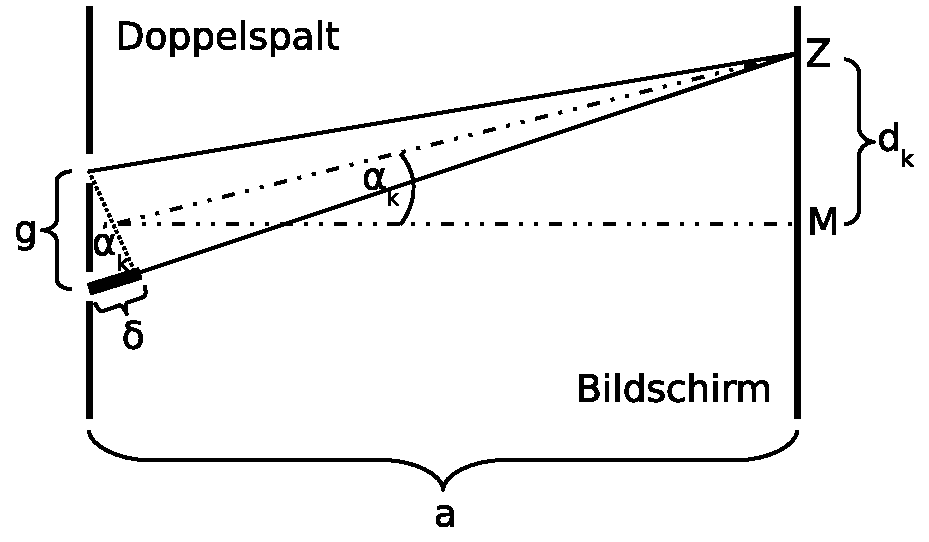
\includegraphics[width=0.7\textwidth]{praktika/mat_praktika/beugung_aufbau01}
 	\caption{Skizze zum Versuchsaufbau zur \emph{Beugung am Doppelspalt} bei geradem Bildschirm zur Erklärung der \textsc{Fraunhofer}-Näherung}
 		\label{img_beugungamdoppelspalt_p}
\end{figure}












\section{Reflektion an einer Halbdurchlässigen Lochplatte - A}


\subsection{Versuch}
\label{kap_reflexion01}

\begin{figure}
	\centering
   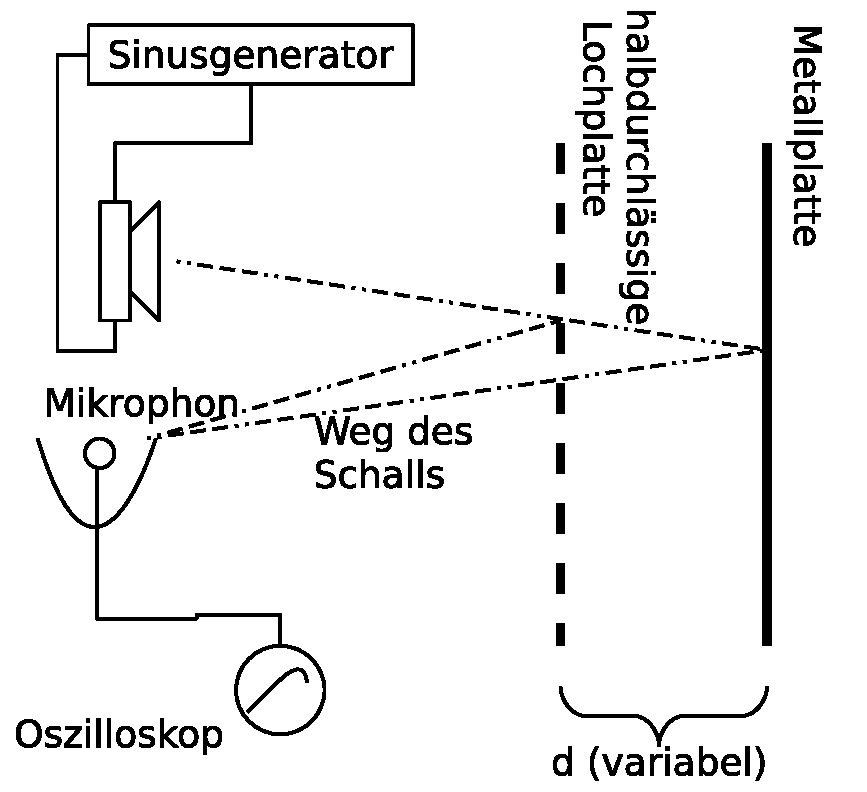
\includegraphics[width=0.6\textwidth]{praktika/mat_praktika/lochplatte}
   \caption{Aufbau des Versuchs über Reflexion an einer halbdurchlässigen Lochplatte.}
   \label{img_aufbau_lochplatte}
\end{figure}


Mikrophon und Lautsprecher werden nebeneinander vor eine Lochplatte gestellt, hinter der eine feste Metallplatte ist. Nun verschiebt man die feste Metallplatte in und entgegen der Richtung zur Lochplatte.




\subsection{Beobachtung}




Verschiebt man die feste Metallplatte in und entgegen der Richtung zur Lochplatte, so beobachtet man im Oszilloskop abwechselnd Minima und Maxima.

Bei unserem Aufbau ergaben sich Maxima bei Abständen \(d\) der Platten voneinander:
\[d = \left \{ 3,0cm; 3,75cm; 4,0cm; 4,7cm; 5,3cm; 5,8cm; 6,3cm; 6,8cm\right \}\]


Es ergeben sich dabei jedoch nie ``absolute'' Minima - also eine gerade Linie auf dem Oszilloskop.



\subsection{Auswertung}


Die Minima und Maxima ergaben sich durch Interferenz. In Abbildung \ref{img_aufbau_lochplatte} Sind die Wege des Schalls von Lautsprecher zu Empfänger eingezeichnet (gestrichelt). Der Schall wird also teilweise von der Lochplatte reflektiert und geht direkt weiter zum Mikrophon, teils kann der Schall aber auch durch die Lochplatte hindurch zur zweiten Wand von der er wieder reflektiert wird.\footnote{Beide Reflexionen erfolgen \emph{ohne} Phasensprung} Ein Teil dieses reflektierten Schalls kann durch die Löcher der Lochplatte wieder austreten. Diese Schallwellen addieren sich dann zu den direkt an der Lochplatte reflektierten. Haben diese beiden Schallwellen wenn sie beim Mikrophon eintreffen den Gangunterschied \(\delta = k \cdot \lambda ~~ k = (0; 1; 2; ...)\) so nimmt das Mikrophon ein Maximum war, bei einem Gangunterschied von \(\delta = k \cdot \lambda + \frac{\lambda}{2} ~~ k = (0; 1; 2; ...)\) registriert es ein Minimum.

Bei diesem Aufbau ist der Gangunterschied die Strecke, die der Schall zwischen Lochplatte und Metallplatte verbringt, somit kommt es auch auf den Abstand zwischen Empfänger und Lautsprecher und deren Abstand von der Lochplatte an, wie lange\footnote{also welche Strecke} der Schall zwischen den beiden Wänden Zeit verbringt\footnote{Je weiter Sender und Empfänger voneinander entfernt sind, desto größer wird der Reflexionswinkel und desto länger ist die Strecke des Schalls zwischen den Platten. Der selbe Effekt ergibt sich, wenn Sender und Empfänger näher bei den Platten sind.}. Da Lautsprecher und Empfänger aber sehr weit von den Platten entfernt sind, nahe beieinander stehen und die Löcher der Lochplatte sehr nahe aneinander liegen, kann man näherungsweise davon ausgehen, dass die Schallwellen senkrecht auf die Lochplatte fallen und ebenso senkrecht reflektiert werden. Somit darf man sagen, dass 
\begin{equation}
   \delta = 2 \cdot d
\end{equation}
näherungsweise gilt.\footnote{Der Schall muss den Abstand \(d\) doppelt überwinden (hin und zurück); daher die \(2\)}

Somit könnte man die Wellenlänge des Schalls über den Zusammenhang berechnen
\begin{equation}
  2 \cdot d = k \cdot \lambda ~~ k = (0; 1; 2; ...)
\end{equation}
Problematischerweise kann man über das \(k\) hierbei keine genauen Aussagen machen, weil man bedingt durch den Versuchsaufbau nicht \(d\) für \(k = 1\) einstellen kann (das wären \(4mm\) Abstand) geschweigedenn den Abstand \(d = 0\). Um zu erkennen, für welche \(k\) man also Maxima aufgezeichnet hat, wurden die Entsprechenden Wellenlängen ausgerechnet; dabei wurde unserem ersten Messwert (\(d = 3cm\)) \(k = k_0\) zugeordnet, dem nächsten Messwert \(k = k_0 + 1\) usw. Daraus wurden die jeweils resultierenden Wellenlängen berechnet und von diesen dann die Abweichung voneinander. Nun wurde der Wert \(k_0\) so lange verändert, bis die Abweichung der errechneten Wellenlängen minimal war; das ergab sich für \(k_0 = 9\).  In Tabelle \ref{tab_lochplatte_wellenlaenge} auf S. \pageref{tab_lochplatte_wellenlaenge} ist zusammengefasst, was sich für unsere Messwerte somit ergibt.


\begin{table}
\centering
\begin{tabular}{l|l|l|l}
\(k\)	&~~~	\(d\) [mm]	&~~~	\(\lambda\) [mm]	&~~~	\(prozentuale Abweichung\)\\
\hline
9	&~~~	30	&~~~	6,67	&~~~	18,3\\
10	&~~~	37,5	&~~~	7,5	&~~~	8,09\\
11	&~~~	40	&~~~	7,27	&~~~	10,87\\
12	&~~~	47	&~~~	7,83	&~~~	4\\
13	&~~~	53	&~~~	8,15	&~~~	0,08\\
14	&~~~	58	&~~~	8,29	&~~~	-1,54\\
15	&~~~	63	&~~~	8,4	&~~~	-2,94\\
16	&~~~	68	&~~~	8,5	&~~~	-4,17\end{tabular}
\caption{Aus unseren Verschiebungen \(d\) errechnete Wellenlängen und deren prozentuale Abweichung vom anfangs bestimmten Wert}
\label{tab_lochplatte_wellenlaenge}
\end{table}

Für \(k = 13\) wurde die Wellenlänge sehr genau bestimmt. Es ist hier ersichtlich, dass bei größeren Abständen \(d\) die Abweichung verhältnismäßig kleiner ist, als bei kleineren Abständen; ein kleiner Messfehler beim Abstand wird einerseits durch eine größere Zahl \(k\) geteilt und macht andererseits nur einen kleineren Prozentsatz von der gemessenen Länge aus. Außerdem fällt der verfälschende Anteil der Näherung geringer aus, je größer die Plattenabstände sind.


\subsection{Reflektionsanteil - A}
\label{kap_reflektionsanteil01}


Ein totales Minimum kann man nur dann beobachten, wenn die beim Mikrophon einlaufende Welle 
\begin{enumerate}
   \item[a)] einen Gangunterschied von \(\delta = \frac{\lambda}{2}\) hat und 
   \item[b)] genau die gleiche Amplitude.
\end{enumerate}

Reflektiert die Lochplatte \(40\%\) des Schalls direkt, so dürfte das vermutlich nicht reichen, damit sich ein absolutes Minimum bilden kann; schließlich werden von den \(60\%\), die die Lochplatte passieren nach der Reflexion nochmal \(40\%\) zur Metallplatte zurückgeworfen. Bei einer anfänglichen Intensität von \(I_0\) erreichen also \(0,4 \cdot I_0\) das Mikrophon direkt und \(0,6 \cdot 0,4 \cdot I_0 = 0,24 \cdot I_0\) erreichen das Mikrophon über eine einzige Reflektion an der Metallplatte; also nur etwas mehr als die Hälfte.

Was hierbei nicht einbezogen ist, sind
\begin{enumerate}
\sloppy   
   \item Der Schall verliert an Intensität, wenn er sich ausbreitet (reziprok kubisch). Da der Abstand \(2 \cdot d = \delta\), den der Schall auf seinem weiteren Weg zusätzlich  nehmen muss, verhältnismäßig klein ist, dürfte das nicht weiter ins Gewicht fallen.
   
   \item Möglicherweise ergeben sich zwischen Loch- und Metallplatte Interferenzphänomene (bspw. eine Stehende Welle), die dann mehr reflektieren kann wenn sie eine Weile angeregt wurde
   
   \item Der Schall, der einmal an der Metallwand reflektiert wurde und von der Lochplatte wieder zurückgeworfen wird, tritt nach einer erneuten Reflektion zu \(60\%\) wieder aus; es treten also \(0,6 \cdot 0,4 \cdot 0,6 \cdot I_0 = 0,114 \cdot I_0\) im nächsten ``Zyklus'' zusätzlich aus und somit tritt nach \(n\) ``Zyklen'' Die Intensität \(0,4^n \cdot 0,6^n \cdot I_0\) aus; Integriert man diese Funktion, so ergibt sich eine maximal austretende Intensität von ca. \(0,316 \cdot I_0\), somit also immer noch weniger als die reflektierten \(40\%\).
\end{enumerate}




\subsection{Mögliche Erklärungen für die Abweichung}
\label{kap_abw02}

Siehe hierzu auch Kap. \ref{kap_abw01} auf S. \pageref{kap_abw01}

\begin{description}
\sloppy
   \item[Wellenlänge] Möglicherweise wurde die Wellenlänge nicht präzise bestimmt; einmal durch Ablesefehler am Oszilloskop oder durch Verwendung der falschen Schallgeschwindigkeit
   
   \item[Abstand] Der Abstand wurde vermutlich nicht genau gemessen; schließlich kam es hierbei auf Millimeter an und man konnte ein Lineal nicht sinnvoll anlegen...
   
   \item[Maxima bestimmen] Es war nicht eindeutig, wann genau man ein Maxima antraf
   
   \item[Näherung] Es gilt bei den Werten zu bedenken, dass die errechneten Werte nur aus einer \emph{Nährungsformel} bestimmt wurden. Schließlich taucht in den Berechnungen weder der Abstand Mikrophon-Lautsprecher noch der Abstand Mikrophon-Lochplatte oder der Abstand der Löcher der Lochplatte auf. Möglicherweise würden unsere Messwerte mit einer präzieseren Berechnung exaktere Ergebnisse liefern.
   
   \item[Parallelität] Möglicherweise waren die beiden Platten nicht vollkommen parallel ausgerichtet oder waren uneben; so ergibt sich logischerweise unterschiedliche Abstände zwischen den Platten an verschiedenen Orgen.
\end{description}






\section{Reflekion an einer Halbdurchlässigen Lochplatte - B}



\subsection{Versuch}

\begin{figure}
	\centering
	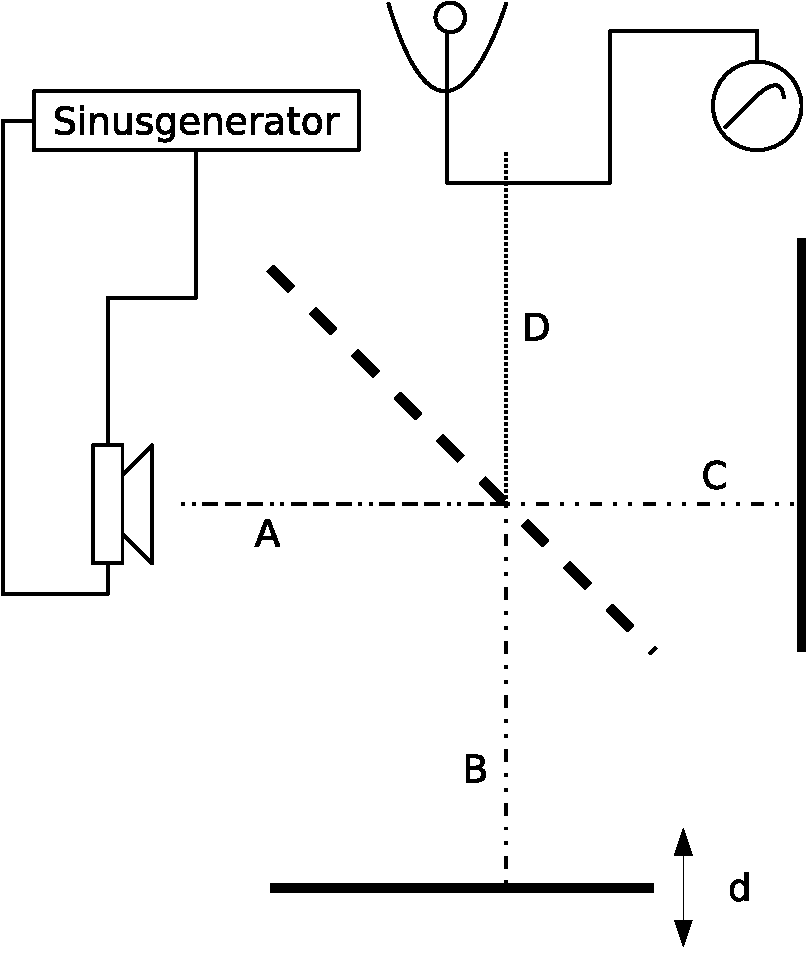
\includegraphics[width=0.5\textwidth]{praktika/mat_praktika/doppellochplatte}   
	\caption{Versuchsaufbau zur Bestimmung der Wellenlänge durch teilweise Refelxion an einer Lochplatte (Zur Zeichenerklärung siehe Abb. \ref{img_aufbau_lochplatte}, S. \pageref{img_aufbau_lochplatte})}
	\label{img_aufbau_doppellochplatte}
\end{figure}


Auf eine schräge Lochplatte werden Schallwellen geworfen. Sie werden teilweise nach unten\footnote{Richtungsangaben beziehen sich auf die Skizze in Abb. \ref{img_aufbau_doppellochplatte} auf S. \pageref{img_aufbau_doppellochplatte}} reflektiert, können auch teilweise nach rechts weiterlaufen. Sowohl unten als auch rechts stehen Metallplatten senkrecht zur Ausbreitungsrichtung des Schalls und reflektieren diesen. Über der Lochplatte befindet sich ein an ein Oszilloskop angeschlossenes Mikrophon, mit dem man die Intensität der Schallwellen\footnote{das Mikrophon ist druckempfindlich} bestimmen kann. Die Schallwellen die rechts reflektiert wurden können zum Mikrophon reflektiert werden, die Schallwellen von unten können die Lochplatte zum Mikrophon passieren. Eine der beiden Metallplatten (in unserem Aufbau die untere) lässt sich dabei parallel zur Schallausbreitungsrichtung verschieben. Immer wenn man am Oszilloskop ein Maximum erkennen kann, misst man, wie weit diese Platte verschoben wurde.



\subsection{Beobachtungen}

Es ergeben sich auf dem Oszilloskop abwechselnd Minima und Maxima; die Minima sind manchmal fast nur eine Gerade auf dem Oszilloskop.

Bei den Abständen \(d\) von einer beliebigen Ausgangslage erkennt man Maxima auf dem Schirm:
\[d = \left \{0mm; 6,5mm; 9mm; 12mm; 23mm; 25mm; 30mm; 37mm; 41mm; 46mm; 50mm \right \} \]





\subsection{Auswertung}


Die Maxima ergeben sich wieder bei einem Gangungerschied der Schallwellen von \(\delta = k \cdot \lambda ~~ k = (0; 1; 2; ..)\). Bei der Reflektion an der Lochplatte nimmt eine Schallwelle den Weg B\footnote{Bezogen auf die Skizze in Abb. \ref{img_aufbau_doppellochplatte} auf S. \pageref{img_aufbau_doppellochplatte}}, die andere den Weg C; vorher nehmen sie einhellig den Weg A. Nachdem die Schallwellen an den Metallplatten reflektiert wurden, nehmen sie nach anschließender Reflektion bzw. Passierung\footnote{Der Akt des Hindurchgelangens ohne Reflektion} der Lochplatte wieder einhellig den Weg D. Auf diesem kommt es nun zu Überlagerungen.

Den Gangunterschied kann man also berechnen, indem man jeweils das Doppelte der Strecken B und C voneinander abzieht\footnote{Das Doppelte deswegen, weil der Schall ja sowohl den Weg hin als auch zurück nehmen muss.}. In der Nullstellung (\(d = 0mm\)) ist dieser Gangunterschied offenslichtlich ein Ganzzahliges Vielfaches der Wellenlänge; welches Vielfache (\(k\)) ist dabei nicht von Bedeutung.

Wir mussten die Metallplatte durchschnittlich um \(d_1 = 4,33mm\) bewegen\footnote{Dabei sind die Werte in zwei Gruppen aufgeteilt; bis einschl. \(12mm\) und ab \(23mm\) - hier wurden offensichtlich einzelne Werte übersprungen}. Um den Faktor \(k\) um eins zu erhöhen wurde die Platte also durchschnittlich um \(4,33mm\) bewegt; somit haben wir durchschnittlich einen Gangunterschied von \(2 \cdot 4,33mm = 8,66mm\) erzeugt. Da wir immer von Maximum zu Maximum gemenssen haben, müsste dieser Gagnunterschied mit der Wellenlänge des Schalls übereinstimmen. 

In der Tat haben wir eine Abweichung von ca. \(-6,1\%\) zu verzeichnen.





\subsection{Mögliche Erklärungen für die Abweichung}

Siehe hierzu auch Kap. \ref{kap_abw01} auf S. \pageref{kap_abw01} und Kap. \ref{kap_abw02} auf S. \pageref{kap_abw02}.


\begin{description}
   \item[Neigung] Möglicherweise war die Lochplatte nicht genau im \(45^o\) Winkel zu den reflektierenden Platten geneigt.
 \end{description}




\subsection{Reflektionsanteil - B}

Vgl. Argumentation in Kap. \ref{kap_reflektionsanteil01} auf S. \pageref{kap_reflektionsanteil01}


Bei diesem Versuch wird von einer Ausgangsintensität \(I_0\) \(40\%\) nach unten reflektiert, von diesen \(40\%\) können \(60\%\) die Lochplatte passieren, der Rest wird in Richtung des Lautsprechers zurückgeworfen. Über die Untere Platte gelangen also \(0,4 \cdot 0,6 \cdot I_0 = 0,24 \cdot I_0\) an das Mikrophon.

Passiert der Schall anfangs die Lochplatte, so nehmen \(60\%\) davon den Weg C. Von diesen \(60\%\) werden anschließend \(40\%\) in Richtung des Mikrophons reflektiert. Über diese Platte gelangen also \(0,6 \cdot 0,4 \cdot I_0 = 0,24 \cdot I_0\) an das Mikrophon.

Da aus beiden ``Schallwegen'' die selbe Intensität (und damit der selbe Druck) ans Mikrophon gelangt, ist es möglich, dass sich bei einem Gangunterschied von \(\delta = k \cdot \lambda + \frac{\lambda}{2} ~~ k = (0; 1; 2; ...)\) die Wellen völlig auslöschen; es ergibt sich also ein absolutes Minimum.


Dieses Absolute Minimum ist mit dem Aufbau in Kap. \ref{kap_reflexion01} auf S. \pageref{kap_reflexion01} nicht erreichbar.


Es gilt jedoch zu beachten, dass folgender Aspekt \emph{nicht} berücksichtigt wurde:
\begin{itemize}
   \item Der Schall verliert bei seiner Ausbreitung an Intensität (reziprok kubisch). Ist also eine der beiden Strecken B oder C deutlich länger, so dürfte diese Abnahme schon dazu führen, dass sich kein absolutes Minimum mehr bilden kann.
\end{itemize}




% \begin{appendix}
% \section{Anhang}
%   \textbf{\textit{\large Berechnung der Abweichung}}
%     
%     Um die Abweichungen zu berechnen wurde folgende Formel verwendet: 
%       
% \begin{equation}
% 100 \cdot \frac{w_g - w_l}{w_l}
% \end{equation}
% 
% Dabei ist \(w_g\) der gemessene Wert und \(w_l\) der errechnete bzw. Literaturwert.
% 
% 
% \end{appendix}









%\end{document}
